% !TeX spellcheck = en_US

\chapter{System Design}
\label{ch:system}

\section{Distributed Architecture}
\label{sec:arch}

In this chapter, we are going to present technical details of our  \textit{Mono3d} solution.
We will start by laying out the high-level architecture, as displayed in Figure~\ref{fig:mono3d-highlevel}.

\begin{figure}[htb]
    \centering
    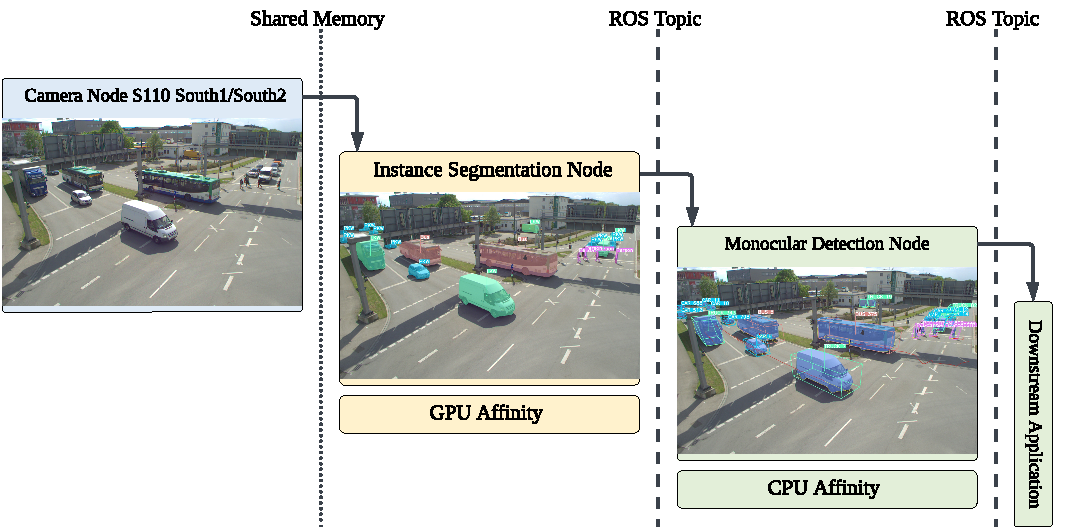
\includegraphics[width=\linewidth]{figures/mono3d-pipeline-highlevel}
    \caption{High-level sketch of the implemented \textit{Mono3d} solution. The Camera Driver Node publishes camera frames to Shared Memory. They are picked up from there by the $2D$ Instance Segmentation node, which requires a machine with strong GPU resources. The detected instances, including their instance masks, are published for each frame via \textit{ROS}, and received by the $3D$ detector node, which does not require a GPU.}
    \label{fig:mono3d-highlevel}
\end{figure}

We have divided our \textit{Mono3d} architecture into three independent process nodes.
A camera driver node, a $2D$ instance segmentation node, and a $3D$ detection node.\ The camera driver node publishes full-resolution $1920p$ RGB image frames at $60Hz$, requiring a throughput of (roughly) $360 \text{MiB}$ per second.
This makes shared memory a good transport medium.
For our solution, we make use of the \textit{Eclipse eCAL} shared memory library \footnote{\hyperlink{https://eclipse-ecal.github.io/ecal/index.html}{https://eclipse-ecal.github.io/ecal/index.html}} to facilitate the communication of camera frames.
The frames are continuously received by the the $2D$ Instance Segmentation node, which is bottlenecked by the performance of the used GPU.
From there, the instance masks of detected objects are published to downstream processes via \textit{ROS}.
In this setup, the second stage our two-stage monocular $3D$ detector is just another consumer of the detected $2D$ instances \textemdash many other consumers may exist for different purposes.
In the second detector stage (the $2D \rightarrow 3D$ lifting stage), $2D$ instance detections are received via ROS and annotated with hypotheses regarding their $3D$ pose.
Again via \textit{ROS}, these $3D$ detections are then broadcast to downstream applications, such as sensor fusion, visualization, or an autonomous vehicle.
This separation of the detection pipeline into multiple concurrent, networked processes offers numerous advantages:

\begin{enumerate}
    \item \textbf{Increased robustness}: A distributed multiprocess solution enhances system robustness by enabling fault tolerance and redundancy.\ When a process fails or encounters an error, other processes in the system can continue to function, minimizing the impact of the failure.\ This capability to recover and adapt to faults makes the overall system more reliable, preventing single points of failure from causing widespread disruptions.
    \item \textbf{Separation of functional concerns}: In a distributed system, each process can focus on a specific functionality, promoting modularity and maintainability.\ This separation of concerns simplifies the design and development of the system, making it easier to understand, debug, and extend.\ It also facilitates reusability, as individual components can be easily replaced or integrated into other systems without affecting the overall system's functionality.
    \item \textbf{Improved assignment of hardware}: The networked solution allows for better resource allocation and hardware utilization.\ By spreading tasks across multiple processes and physical machines, the system can allocate specific resources, such as GPUs, to each process based on its requirements.\ This flexibility enables more efficient use of available hardware, reducing resource contention and potential bottlenecks, while also providing the opportunity to optimize cost and energy consumption.
    \item \textbf{Increased performance}: The asynchronous process collaboration enables parallelism, allowing multiple tasks to be executed concurrently.\ This parallel execution can significantly improve the overall performance and throughput of the system.\ By leveraging the processing capabilities of multiple machines, distributed systems can handle larger workloads and scale more effectively than a single-process system.\ Additionally, this architecture allows for load balancing, which can help distribute work evenly and prevent overloading individual components.
\end{enumerate}

Natural tradeoffs of this architecture are increased complexity and a nonzero communication overhead, as data must be serialized and deserialized into discrete messages.
However, the advantages of the distributed approach tend to outweigh the negatives, especially where scalability is a concern.

% ----------------------------------------------------

\section{The 2D Object Detector}
\label{sec:segmentation}

The $2D$ Object Detector receives camera input frames from a camera driver node via shared memory.
It uses an off-the-shelf Object Recognition and Instance Segmentation solution (currently \textit{YOLOv7/Blendmask}~\cite{wang2022yolov7, chen2020blendmask}) to detect $2D$ bounding boxes and pixel masks of Vehicles and Vulnerable Road Users (VRUs).
As the performance of such an object detection solution inversely scales to the square of the input image resolution, the $2D$ object detector may also downsize the incoming frames from $1920*1200$ to $1280*800$ or even $640*400$ using \textit{OpenCV}~\cite{opencv_library}.
The performance impact of this downscaling is further explored in Section~\ref{sec:performance}.
As the instance masks of detected objects must be efficiently passed via \textit{ROS} messages, bit packing~\cite{5219512} is used to efficiently serialize the pixel mask arrays for each instance.
Earlier work within Providentia~\cite{leonthesis} went so far as to conclude that the throughput demands of the instance masks is far too high for a distributed solution to be viable, but this turned out to be overly pessimistic.
Each detected instance consists of a pixel mask, a $2D$ screen-space bounding box, and an assigned object category.
As we are currently using the \textit{YOLOv7} detector which was trained on the \textit{MS COCO} dataset, our $2D$ object detector is able to distinguish between six different object classes: \texttt{CAR}, \texttt{BUS}, \texttt{TRUCK}, \texttt{MOTORCYCLE}, \texttt{BICYCLE}, \texttt{PEDESTRIAN}.
The \texttt{VAN}, \texttt{EMERGENCY\_VEHICLE}, and \texttt{OTHER} classes from the \textit{A9 Dataset} cannot yet be recognized.

\section{The 3D Object Detector}
\label{sec:mono3doverview}

In the second stage of our \textit{Mono3d} solution, $2D$ object detections are received as an array $D^{2D}_t$ of detection triplets for each frame:

\[
    D^{2D}_t = \{ (\mathtt{category}_n, \overrightarrow{\mathtt{bbox}}^{2D}_n, \mathtt{mask}_n)^{n < N}_{n=0}\}
\]

The per-frame detection array is received in a single \textit{ROS} topic update message from the upstream $2D$ object recognition node.
Now, the task of the receiving $3D$ object detector is to generate a best-effort physical pose hypothesis for each $2D$ detection.
The estimated $3D$ pose must include the objects bottom-center $\overrightarrow{\mathtt{xyz}}$ position, its \texttt{length}, \texttt{width}, and \texttt{height} in meters, and its \texttt{yaw} heading angle.
The full process of estimating these pose parameters from a $2D$ detection triplet is illustrated in Figure~\ref{fig:mono3d-lowlevel}.

\begin{figure}[htb]
    \centering
    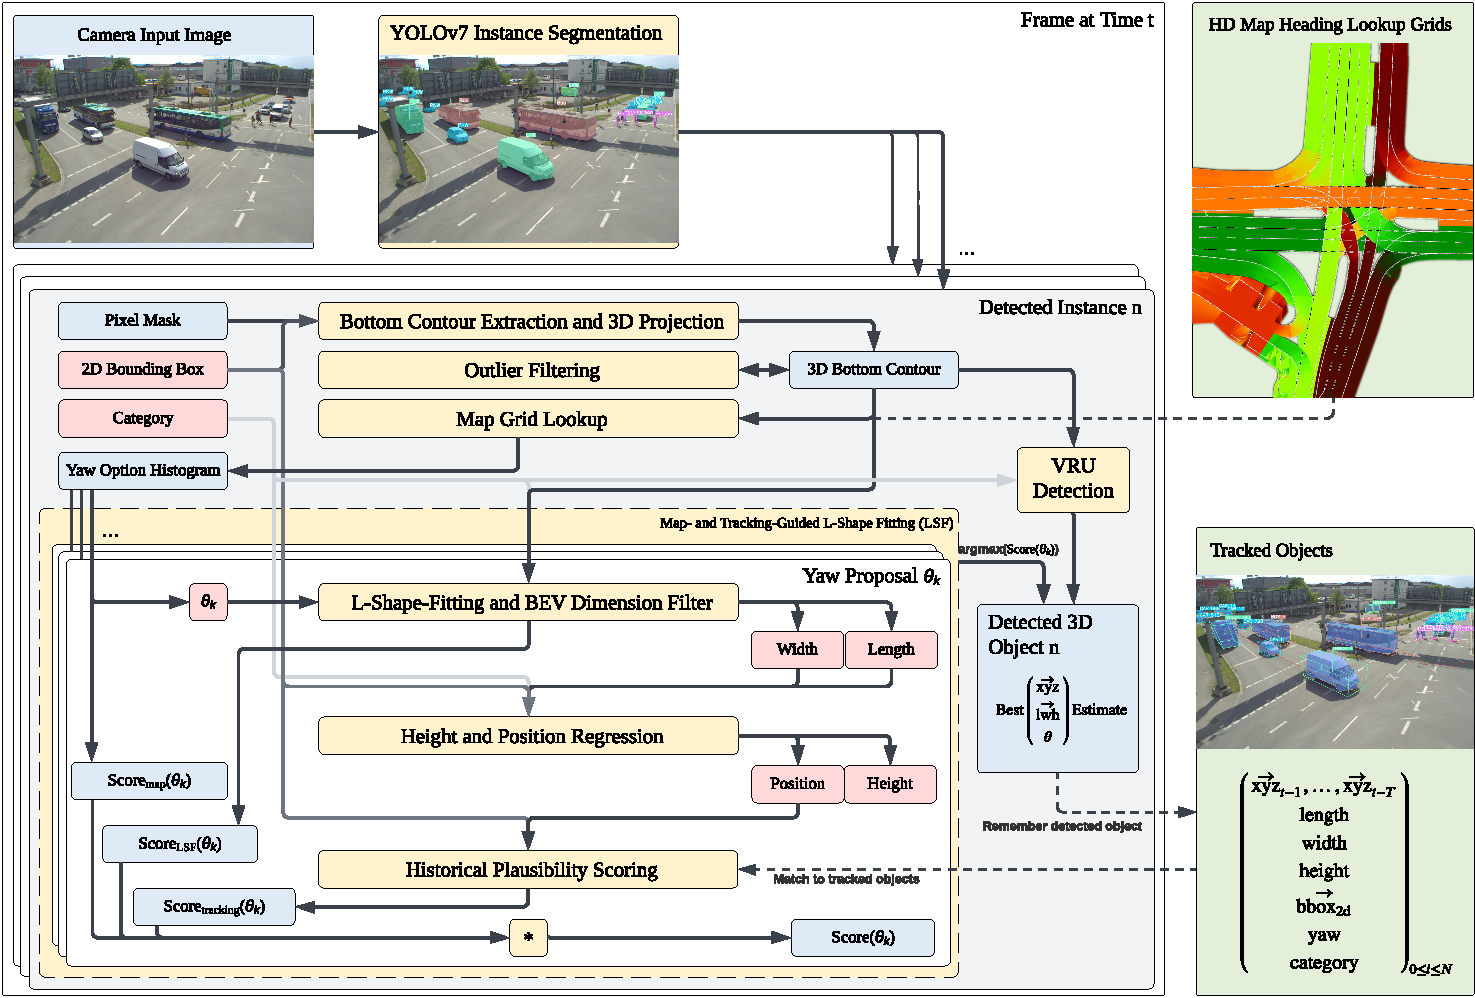
\includegraphics[width=\linewidth]{figures/mono3d-pipeline-lowelevel}
    \caption{Low-level illustration of our \textit{Mono3d} pipeline. To determine a $3D$ pose for a non-VRU $2D$ object instance, its associated pixel mask and category are passed through six processing steps: \textbf{(1)} \textit{Bottom Contour Projection}, \textbf{(2)} \textit{Outlier Filtering}, \textbf{(3)} \textit{Map Grid Yaw Option Lookup}, \textbf{(4)} \textit{L-Shape-Fitting}, \textbf{(5)} \textit{Height and Position Regression}, \textbf{(6)} \textit{Historical Plausibility Scoring}. \textbf{Legend:} Blue boxes mark normal I/O data, red boxes mark I/O variables which are primary components of a final pose hypothesis. Yellow boxes mark processes. Green boxes with dashed arrows mark auxiliary data flow which is not restricted to the scope of the current frame.}
    \label{fig:mono3d-lowlevel}
\end{figure}

The high-level process which turns the instance mask and category inputs into a 3D pose hypothesis for each $2D$ detection is summarized in the following:
First, the instance mask is filtered to extract its bottom contour (see Section~\ref{sec:botcont}).
This yields a line of $2D$ pixel coordinates $\{\overrightarrow{uv}_i\}_{i=0}^{i < N}$.
These are projected into $3D$ map space using a simple raycast, whereas the $z$ (altitude) coordinate is set to 0.
The resulting $3D$ point cloud $\{\overrightarrow{\text{xyz}}_i\}_{i=0}^{i < N}$ is optionally filtered using the \textit{DBSCAN} algorithm to remove outlier points.
If the category of the detected object is that of a \textit{Vulnerable Road User} such as a pedestrian or bicycle, the bottom contour will be converted to a $3D$ pose estimation with a special algorithm as explained in Section~\ref{sec:pedcyc}.
Otherwise, the \textit{HD Map Lookup Grids} (see Section~\ref{sec:hdmapgrids}) are queried at the positions of the $3D$ points.
This query provides a set of $\{(\mathtt{lane\_id}_k, \theta_k)\}_{k=0}^{k<K}$ for each point where the bottom contour touches a particular lane's surface.
These tuples are averaged and aggregated into a histogram per unique \texttt{lane\_id} (see Section~\ref{sec:hdmaplsf}).
This histogram provides $\theta_k$ values with associated confidences $\text{Score}_\text{map}(\theta_k)$ derived from the number of bottom contour points which touch the associated lane.

Thereafter, for each yaw option $\theta_k$, the \textit{L-Shape-Fitting (LSF)} algorithm is used to calculate the physical length and width of the given bottom contour assuming the given $\theta_k$. \textit{LSF} also returns an error score $\text{Score}_\text{lsf}(\theta_k)$ indicating $p(\theta_k|\{\overrightarrow{\text{xyz}}_{0 \leq i < N}\})$ (see Section~\ref{sec:botcontlsf}).
The proposed length and width values are also sanity-checked against limits per the detected object category.
Using these assumed spatial extents, the spatial position and height can be regressed from the $2D$ instance bounding box (see Section~\ref{sec:sizeandpos}).

Finally, the $2D$ instance bounding box is also matched against historical detections via \textit{SORT} object tracking to find previous detections of the same vehicle.
According to the historical vehicle trajectory, a $\theta_k$ proposal also receives a historical plausibility/fitness score $\text{Score}_\text{track}(\theta_k)$ (see Section~\ref{sec:trackinglsf}).
Multiplied together, the three scores $\text{Score}_\text{map}(\theta_k)$, $\text{Score}_\text{lsf}(\theta_k)$ and $\text{Score}_\text{map}(\theta_k)$ yield the final $\text{Score}(\theta_k)$.
Now, for the object in question, we hypothesize that the best $\theta_k$ yaw choice (and associated pose parameters) is the one which finally receives the highest score.
This is calculated for every detected $2D$ object to perform the $2D \rightarrow 3D$ lifting operation.

The following sections of this chapter serve to explain each step in detail.

% ----------------------------------------------------

\section{Bottom Contour Extraction and Filtering}
\label{sec:botcont}

In the first processing step for each $2D$ detection, the detection's pixel mask is converted to a $3D$ bottom contour.
We can express the image mask for detection $n$ as a function $\mathtt{Mask}: \mathbb{N}^2 \rightarrow \mathbb{B}$, as it maps uv pixel coordinates to a boolean value which indicates whether the object occupies the given pixel.
The pixel coordinates are modeled as $\overrightarrow{uv}$ vectors with $u$ indicating the pixel column, $v$ indicating the pixel row, and $\overrightarrow{00}$ as the top-left image corner.
In this model, the $2D$ bottom contour points $B^n_{2D}$ are extracted as follows:

\[
    B^n_{2D}=\{\overrightarrow{uv}|\mathtt{Mask}_n(\overrightarrow{uv}) \land \neg \mathtt{Mask}_n( \begin{pmatrix}u\\v+1\end{pmatrix}) \}
\]

In practice, the operation is realized using a \textit{numpy}~\cite{harris2020array} \textit{argmax} call.
Successively, the $2D$ bottom contour points are projected into $3D$ map space via a raycast operation.
We assume that the ground plane is located at $z=0$, $P$ is the camera's intrinsic (projection) matrix, $R$ is the camera's spatial rotation and $T=\begin{pmatrix} T_x & T_y & T_z \end{pmatrix}$ is the camera's spatial translation relative to the ground plane.
Therefore, the bottom contour $3D$ ground points $B^n_{3D,\text{ground}}$ are calculated as follows:

\begin{gather*}
    B^n_{3D,\text{init}}=\bigcup_{\overrightarrow{uv} \in B^n_{2D}} \{\overrightarrow{\text{xyz}} | \overrightarrow{\text{xyz}} = R^T * P^{-1} * \overrightarrow{uv1}\}\\
    B^n_{3D,\text{ground}}=\bigcup_{\overrightarrow{\text{xyz}} \in B^n_{3D,\text{init}}} \{\overrightarrow{\text{xyz}_\text{ground}} | \overrightarrow{\text{xyz}_\text{ground}} = T + \overrightarrow{\text{xyz}} * -T_z/z\}\\
\end{gather*}

This point set is then filtered using the \textit{DBSCAN}~\cite{schubert2017dbscan} algorithm to get rid of outlier points which do not belong to the true $3D$ bottom outline.

\section{Detection of Vulnerable Road Users}
\label{sec:pedcyc}

\textit{Vulnerable Road Users (VRUs)}, such as pedestrians or bicyclists, receive special treatment in our \textit{Mono3d} pipeline.
This is, because several assumptions which are made for optimized road vehicle detection are not valid for VRUs:

\begin{enumerate}
    \item \textbf{Legal Heading Assumption}: For road vehicles, the monocular detector makes use of the HD map to derive yaw options from legal traffic flow directions.\ This is not possible for bicyclists or pedestrians, as these often move along unmapped territory beyond the road, and perpendicular to normal traffic directions on mapped vehicle lanes.
    \item \textbf{Box Shape Assumption}: Cars, trucks and other motorized road users usually exhibit an instance mask bottom contour shape which indicates the occupied ground area of the object, and therefore allows for L-Shape-Fitting as an effective algorithm to derive the object's length and width.\ This is usually not the case for pedestrians and bicycles, which might have major errors in the projected bottom contours (see Figure~\ref{fig:mono3d-vru}).
\end{enumerate}

For these reasons, we have implemented a simplified detection flow for VRUs: We do not attempt to detect their orientation, instead they are always assigned $\theta=0$.
Furthermore, their dimensions are set to fixed values.
The only variables which remain to be estimated are the VRU's BEV coordinates.
This is done by averaging the positions of $10$ percent of the road user's bottom contour $B^n_{3D,\text{ground}}$ points, which are closest to the camera from the BEV perspective.

The reasoning for this strategy is illustrated in Figure~\ref{fig:mono3d-vru}:
The camera $C$ detects pedestrian $A$ and cyclist $B$.
The projection of their instance mask bottom contour (highlighted in red) to the ground is highlighted in blue.
Points on the $3D$ bottom contour which are close to the camera BEV position and therefore considered to estimate the position of $A$ and $B$ are respectively shown.

\begin{figure}[htb]
    \centering
    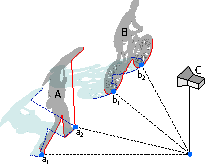
\includegraphics[width=0.8\linewidth]{figures/vru-detection}
    \caption{Illustration of our proposed solution for VRU detection. Camera $C$ observes pedestrian $A$ and cylist $B$. Their 2D bottom contour outline is highlighted in red, the projection of the outline to the ground is highlighted in dashed blue lines. Only the highlighted points on the respective bottom contour projections which remain close to the camera may be considered to estimate the position of $A$/$B$.}
    \label{fig:mono3d-vru}
\end{figure}

\section{Bottom Contour L-Shape Fitting}
\label{sec:botcontlsf}

The process of estimating $\theta$, width and length for motorized road vehicles is realized using the \textit{L-Shape-Fitting (LSF)} algorithm~\cite{zhang2017efficient} with an augmented score calculation function.
From the standard LSF implementation, we use the \textit{Variance} criterion, as it was demonstrated to perform the best in the original paper.
The value of the LSF variance score $\mathtt{Variance}_{\text{LSF}}(\theta_k)$ is in the range of $[-\infty, 0]$.
We convert this value to the range of $[0, 1]$ as $\text{Score}_\text{lsf}(\theta_k)=1 / (1 - \mathtt{Variance}_{\text{LSF}}(\theta_k))$.
Then we combine it using multiplication with the map confidence score (see Section~{\ref{sec:hdmaplsf}}) and the historical plausibility score (see Section~{\ref{sec:trackinglsf}}), to arrive at the final  $\text{Score}(\theta_k)$.

% ----------------------------------------------------

\section{HD Map Lookup Grids}
\label{sec:hdmapgrids}

HD Map Grids \par
Rendering \par
Resolution

\newpage

\newpage

% ----------------------------------------------------

\section{HD-Map-Augmented L-Shape Fitting}
\label{sec:hdmaplsf}

HD Map Grid Lookup - Early \par
Yaw Lookup Histogram \par
Confidence

\newpage

% ----------------------------------------------------

\section{Tracking-Augmented L-Shape Fitting}
\label{sec:trackinglsf}

Historical Plausibility \par
2D Tracking SORT Lookup

\newpage

% ----------------------------------------------------

\section{Joint Height and Position Estimation}
\label{sec:sizeandpos}

L/W/H Dimension Filtering \par
Height Estimation

\newpage

% ----------------------------------------------------

\section{Late HD Map Lookup}
\label{sec:hdmaplate}

HD Map Grid Lookup - Late \par
Tempting, Simple, Bad

\section{3D Tracking}
\label{sec:trackthreed}

3D Tracking \par
LIDAR Label Shifting
